\documentclass[a4paper,14pt]{extarticle}

\usepackage[utf8x]{inputenc}
\usepackage[T1,T2A]{fontenc}
\usepackage[russian]{babel}
\usepackage{hyperref}
\usepackage{indentfirst}
\usepackage{here}
\usepackage{array}
\usepackage{graphicx}
\usepackage{caption}
\usepackage{subcaption}
\usepackage{chngcntr}
\usepackage{amsmath}
\usepackage{amssymb}
\usepackage{pgfplots}
\usepackage{pgfplotstable}
\usepackage[left=2cm,right=2cm,top=2cm,bottom=2cm,bindingoffset=0cm]{geometry}
\usepackage{multicol}

\renewcommand{\le}{\ensuremath{\leqslant}}
\renewcommand{\leq}{\ensuremath{\leqslant}}
\renewcommand{\ge}{\ensuremath{\geqslant}}
\renewcommand{\geq}{\ensuremath{\geqslant}}
\renewcommand{\epsilon}{\ensuremath{\varepsilon}}
\renewcommand{\phi}{\ensuremath{\varphi}}

\counterwithin{figure}{section}
\counterwithin{equation}{section}
\counterwithin{table}{section}
\newcommand{\sign}[1][5cm]{\makebox[#1]{\hrulefill}} % Поля подписи и даты
\graphicspath{{pics/}} % Путь до папки с картинками
\captionsetup{justification=centering,margin=1cm}
\def\arraystretch{1.3}


\begin{document}

\begin{titlepage}	% начало титульной страницы

	\begin{center}		% выравнивание по центру

		\large Санкт-Петербургский Политехнический Университет Петра Великого\\
		\large Институт компьютерных наук и технологий \\
		\large Кафедра компьютерных систем и программных технологий\\[6cm]
		% название института, затем отступ 6см
		
		\huge Метрология, стандартизация и сертификация\\[0.5cm] % название работы, затем отступ 0,5см
		\large Отчет по лабораторной работе №2\\[0.1cm]
		\large <<Регулятор мощности>>\\[6cm]

	\end{center}


	\begin{flushright} % выравнивание по правому краю
		\begin{minipage}{0.30\textwidth} % врезка в половину ширины текста
			\begin{flushleft} % выровнять её содержимое по левому краю

				\large\textbf{Работу выполнил:}\\
				\large Ламтев А.Ю.\\
				\large {Группа:} 23501/4\\
				
				\large \textbf{Преподаватель:}\\
				\large Кошелев С.И.

			\end{flushleft}
		\end{minipage}
	\end{flushright}
	
	\vfill % заполнить всё доступное ниже пространство

	\begin{center}
	\large Санкт-Петербург\\
	\large \the\year % вывести дату
	\end{center} % закончить выравнивание по центру

\thispagestyle{empty} % не нумеровать страницу
\end{titlepage} % конец титульной страницы

\vfill % заполнить всё доступное ниже пространство


\tableofcontents
\newpage

\section{Моделирование схемы в OrCAD Capture}

\subsection{Исходная схема}

На рисунке \ref{pic:scheme} изображена схема регулятора яркости люстры или температуры паяльника. (файл \textbf{Регулятор\_мощности.doc})

\begin{figure}[H]
\begin{center}
	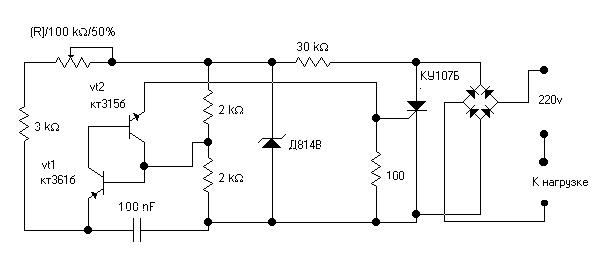
\includegraphics[width=1\textwidth]{scheme}
	\caption{Схема регулятора яркости люстры или температуры паяльника}
	\label{pic:scheme}
\end{center}
\end{figure}

Через мостовую схему на диодах ток идет на резистор 30 кОм, затем напряжение опустится до напряжения стабилитрона Д814В, в качестве которого можно применить любой на 9$\dots$12 вольт, дальше напряжение поступает на переменный резистор 100 кОм и 2 кОм первый соединяется 3 ком и конденсатором 100 nf на этой цепочке образуется на время задерживающая сигнал периодов тока, который подается на эмиттер кт361б при до-стижении напряжения более напряжения двух резисторов по 2 ком транзистор начинает открываться при этом начинает открывать следующий транзистор и тогда ток поступает на тиристор    КУ107б и он откры-вается. При регулировке переменным резистором регулируется яркость лампы или температура паяль-ника. Диодную сборку можно применить любую на напряжение не менее 300 вольт и ток в зависимости от нагрузки например (кц 405 а .. 400вольт 1ампер) или диоды соединенные по мостовой схеме. Тиристор можно заменить на ку208г или другой 300….*** вольт и ток мощнее диодов раза в два. Еще надо чтобы резистор 30 ком был 2 вата.

Через мостовую схему на диодах ток идет на резистор 30 кОм затем напряжение опустится до напряжения стабилитрона Д814В можно применить любой на 9…12 вольт, дальше напряжение поступает на переменный резистор 100 кОм и 2 кОм первый соединяется 3 кОм и конденсатором 100 nf на этой цепочке образуется на время задерживающая сигнал периудов тока , который подается на эмиттер КТ361б при достижении напряжения более напряжения двух резисторов по 2 кОм транзистор начинает открываться при этом начинает открывать следующий транзистор и тогда ток поступает на тиристор КУ107Б и он открывается . При регулировки переменным резистором регулируется яркость лампы или температура паяльника. Диодную сборку можно применить любую на напряжение не менее 300 вольт и ток в зависимости от нагрузки например (КЦ405А - 400 В, 1 А) или диоды соединенные по мостовой схеме. Тиристор можно заменить на КУ208Г или другой 300 В и ток мощнее диодов раза в два подберите на радио рынке сами вам подскажут. Еще надо чтобы резистор 30 кОм был 2 Вт

\subsection{Элементы схемы}

\begin{table}[H]
\begin{center}
	\caption{Транзисторы}
	\def\tabcolsep{10pt}
	\begin{tabular}{|l|l|l|l|l|l|l|}
		\hline
		наименование &
		тип & 
		$I_k$, А &
		$U_\text{кэ}$, В & 
		$P$, Вт & 
		$F$, МГц & 
		$\beta_{min}$ \\ 
		\hline
		КТ315Б &
		n-p-n &
		0.1 &
		20 &
		0.15 &
		250 &
		50 \\
		\hline
		BC846 &
		n-p-n &
		0.1 &
		65 &
		0.33 &
		250 &
		110 \\
		\hline
		КТ361Б &
		p-n-p &
		0.05 &
		20 &
		0.15 &
		250 &
		50 \\
		\hline
		Q2N4250 &
		p-n-p  &
		0.05 &
		25 &
		&
		500 &
		500 \\ 
		\hline
\end{tabular}
\end{center}
\end{table}

\begin{table}[H]
\begin{center}
	\caption{Диоды}
	\def\tabcolsep{10pt}
	\begin{tabular}{|l|l|l|l|}
		\hline
		наименование &
		$I_\text{пр max}$, А &
		$U_\text{обр}$, В &
		$U_\text{пр}$, В \\ 
		\hline
		КЦ405А &
		1 &
		600 &
		4 \\
		\hline
		MUR160 &
		1 &
		600 &
		1.35 \\
		\hline
\end{tabular}
\end{center}
\end{table}

\begin{table}[H]
\begin{center}
	\caption{Стабилитроны}
	\def\tabcolsep{10pt}
	\begin{tabular}{|l|l|l|l|l|}
		\hline
		наименование &
		$U_\text{ст}$, В &
		$I_\text{ст}$, мА &
		$I_\text{ст max}$, мА &
		$R_\text{дифф}$, Ом \\ 
		\hline
		Д814В &
		9---10.5 &
		3 &
		32 &
		12 \\
		\hline
		D1N758 &
		10 &
		20 &
		35 &
		17 \\
		\hline
\end{tabular}
\end{center}
\end{table}

\begin{table}[H]
\begin{center}
	\caption{Тиристоры}
	\def\tabcolsep{4pt}
	\begin{tabular}{|c|c|c|c|c|c|c|c|}
		\hline
		наименование &
		$I_\text{пр ос}$, А &
		$U_\text{пр}$, В &
		$U_\text{вкл}$, В &
		$I_\text{зс}$, мА &
		$U_\text{отп}$, В &
		$t_\text{вкл}$, $\mu$с &
		$t_\text{выкл}$, $\mu$с \\ 
		\hline
		КУ208Г &
		5 &
		2 &
		400 &
		5 &
		5 &
		10 &
		150 \\
		\hline
		MAC228A6 &
		8 &
		2 &
		400 &
		5 &
		10 &
		1.5 &
		\\
		\hline
		MCR729-6 &
		5 &
		1.5 &
		400 &
		10 &
		5 &
		0.4 &
		15 \\
		\hline
\end{tabular}
\end{center}
\end{table}

\subsection{Схема моделирования}

\subsection{Результаты моделирования}

\subsection{Измеряемые величины}

\section{Оценка априорной инструментальной погрешности измерений}

\subsection{Методы измерений}

\subsection{Средства измерений}

\subsection{Погрешность измерений}

\end{document}
